\documentclass[10 pt,a4paper, openany]{article}
%titlepage
\usepackage[hidelinks]{hyperref}
\usepackage[italian]{babel}
\usepackage[T1]{fontenc}
\usepackage[utf8x]{inputenc}
\usepackage{amsfonts}
\usepackage{multicol}
\usepackage{graphicx}
\usepackage{amsmath}
\usepackage{framed}
\usepackage{extarrows}
\usepackage{cancel}
\usepackage{eurosym}
\usepackage{listingsutf8}
\usepackage{lastpage}
\usepackage{rotating} 
\usepackage{multirow}
\usepackage{placeins}
\usepackage{caption}
\usepackage{makecell}
\usepackage{longtable}
\usepackage{array}
\date{}


\usepackage{makeidx}
\makeindex
\usepackage{fancyhdr}
\pagestyle{fancy}
\lhead{
\includegraphics[width=.6cm]{../../../../../file_comuni/immagini/obelisk_sample_02.png}
  Obelix Group}
\chead{}
\rhead{\rightmark }% \leftmark}%da rimettere
\lfoot{}
\cfoot{}
\rfoot{\thepage / \pageref*{LastPage}}
%%%%%%%%%%%%%%%%%%%%%%%%%%%%%%%%%%%%%%
%\usepackage{lipsum}
\usepackage{../../../../../file_comuni/copertina2}
\nomedoc{Verbale interno 2017-09-05}
\versione{v1\_0\_0}
\datacreazione{2017/09/05}
\verifica{Riccardo Saggese}
\approvazione{Nicolò Rigato}
\redazione{Emanuele Crespan \eanche Federica Schifano}
\uso{interno}
\distribuzione{Prof. Tullio Vardanega \eanche Prof. Riccardo Cardin \eanche Red Babel \eanche Gruppo Obelix}
\sommario{Verbale dell'incontro tra i membri del gruppo \emph{Obelix} in data 2017-09-05}


\begin{document}
\paginatitolo
\section{Informazioni sulla riunione}

\begin{itemize}
\item[] Data: 2017-09-05
\item[] Luogo: Torre Archimede - Via Trieste, 63 Padova
\item[] Ora: 10.30
\item[] Durata: 80'
\item[] Partecipanti interni: Obelix
  \begin{itemize}
  \item[] Emanuele Crespan
  \item[] Federica Schifano
  \item[] Nicolò Rigato
  \item[] Riccardo Saggese
  \item[] Silvio Meneguzzo
  \item[] Tomas Mali
 \end{itemize}
\end{itemize}

\section{Argomenti trattati}
\begin{enumerate}
	\item Situazione correzione documenti	
	\item Situazione Demo

	
\end{enumerate}


\section{Decisioni Prese}
\begin{enumerate}
	\item \textbf{VI2.1} I documenti Piano di Qualifica, Norme di Progetto, Analisi dei Requisiti, Definizione di Prodotto sono stati corretti secondo le segnalazioni in seguito al periodo di revisione di Qualifica, manca il calcolo di alcune metriche che sarà svolto nei seguenti giorni.
	I documenti rimanenti tra cui i Manuali sono ancora in fase di completamento
	\item \textbf{VI2.2} La Demo è stata conclusa ed è ora funzionante
	
			\FloatBarrier
			\begin{figure}[ht]
				\centering
				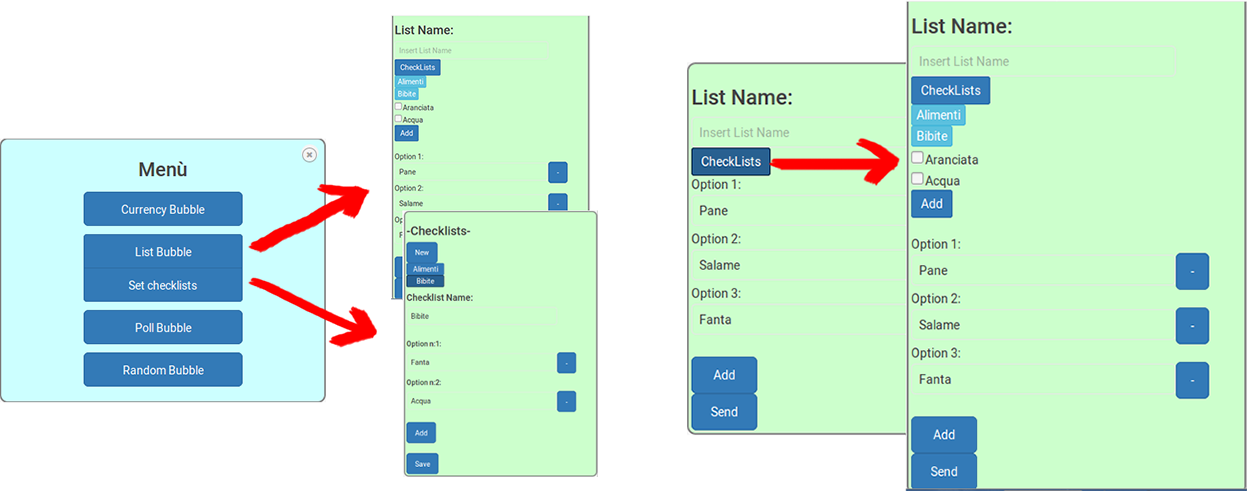
\includegraphics[scale=0.20]{img/demo.png}
				\caption{funzionamento Demo}
			\end{figure}
	

\end{enumerate}


\end{document}